\section{Experiments}
\begin{figure}[t]
  \centering
    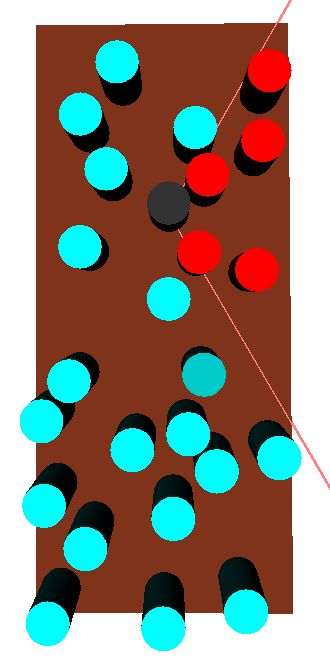
\includegraphics[scale=0.3,angle=90]{images/feature_cone.png}
  \caption{\small{If the target object to be grasped is the black can, we consider the objects
whose centers lie in a cone from angles $-\frac{\pi}{3}$ to $\frac{\pi}{3}$ toward the closest table edge in
our feature computations. These objects are shown here in red.}}
  \label{fig:cone}
\end{figure}

\begin{table}[t]
  \centering
  \vspace{8pt}
  \tabcolsep=0.11cm{
  \begin{tabular}{ccccc}
    \toprule[1.5pt]
      \textbf{\# Cans} & \textbf{System} & \textbf{\% Solved} & \textbf{Avg Time (s)} & \textbf{Avg \# MP Calls}\\
    \midrule[2pt]
      25 & B1 & 96 & 28.7 & 22\\
    \midrule
      25 & B2 & 98 & 30.0 & 21\\
    \midrule
      25 & I0 & 94 & 24.8 & 21\\
    \midrule
      25 & I1 & 94 & 28.5 & 19\\
    \midrule
      25 & I2 & 100 & 21.0 & 18\\
    \midrule[1.5pt]
      30 & B1 & 74 & 48.9 & 29\\
    \midrule
      30 & B2 & 80 & 48.0 & 29\\
    \midrule
      30 & I0 & 72 & 40.0 & 29\\
    \midrule
      30 & I1 & 76 & 44.2 & 28\\
    \midrule
      30 & I2 & 80 & 42.7 & 30\\
    \midrule[1.5pt]
      35 & B1 & 68 & 24.5 & 15\\
    \midrule
      35 & B2 & 72 & 29.7 & 15\\
    \midrule
      35 & I0 & 74 & 31.1 & 15\\
    \midrule
      35 & I1 & 76 & 22.4 & 14\\
    \midrule
      35 & I2 & 80 & 22.7 & 14\\
    \midrule[1.5pt]
      40 & B1 & 58 & 35.9 & 15\\
    \midrule
      40 & B2 & 64 & 48.0 & 19\\
    \midrule
      40 & I0 & 58 & 54.5 & 22\\
    \midrule
      40 & I1 & 64 & 36.6 & 14\\
    \midrule
      40 & I2 & 76 & 36.9 & 16\\
    \bottomrule[1.5pt]
  \end{tabular}}
  \caption{\small{Percent solved, average overall time, and average number of calls to the motion
planner for baseline 1 (B1), baseline 2 (B2), and our method after iterations 0 (I0), 1 (I1), and 2 (I2).
Iteration 0 evaluates performance before DAgger was run (so just the initial set of 100 demonstrations),
and iterations 1 and 2 are after one and two rounds of DAgger, respectively. Average time and number of
motion planner calls were computed across the subset of environments for which all systems succeeded, which
explains why they do not scale with the number of cans. Time limit: 300s.}}
  \label{table:results}
  % \vspace{-1em}
\end{table}

We evaluate our approach in the can domain, which has cans distributed on a table. We
compare performance with two baselines. Baseline 1 is SFRCRA-14, which uses the
following fixed graph search policy: try 3 times to refine the deepest
node in the PRGraph; if unsuccessful, generate a geometric fact from it, replan (which
creates a child node), and repeat. The number 3 was chosen to trade off between providing
each node a fair opportunity to be refined (which could fail a couple of times if sampling produces
undesirable values), and not spending too much time before giving up and generating a child node to try next.
Baseline 2 is the prior work by Chitnis et al.~\cite{chitnis2015mlpc}, described in Section IV-C.

\begin{figure}[h]
  \centering
    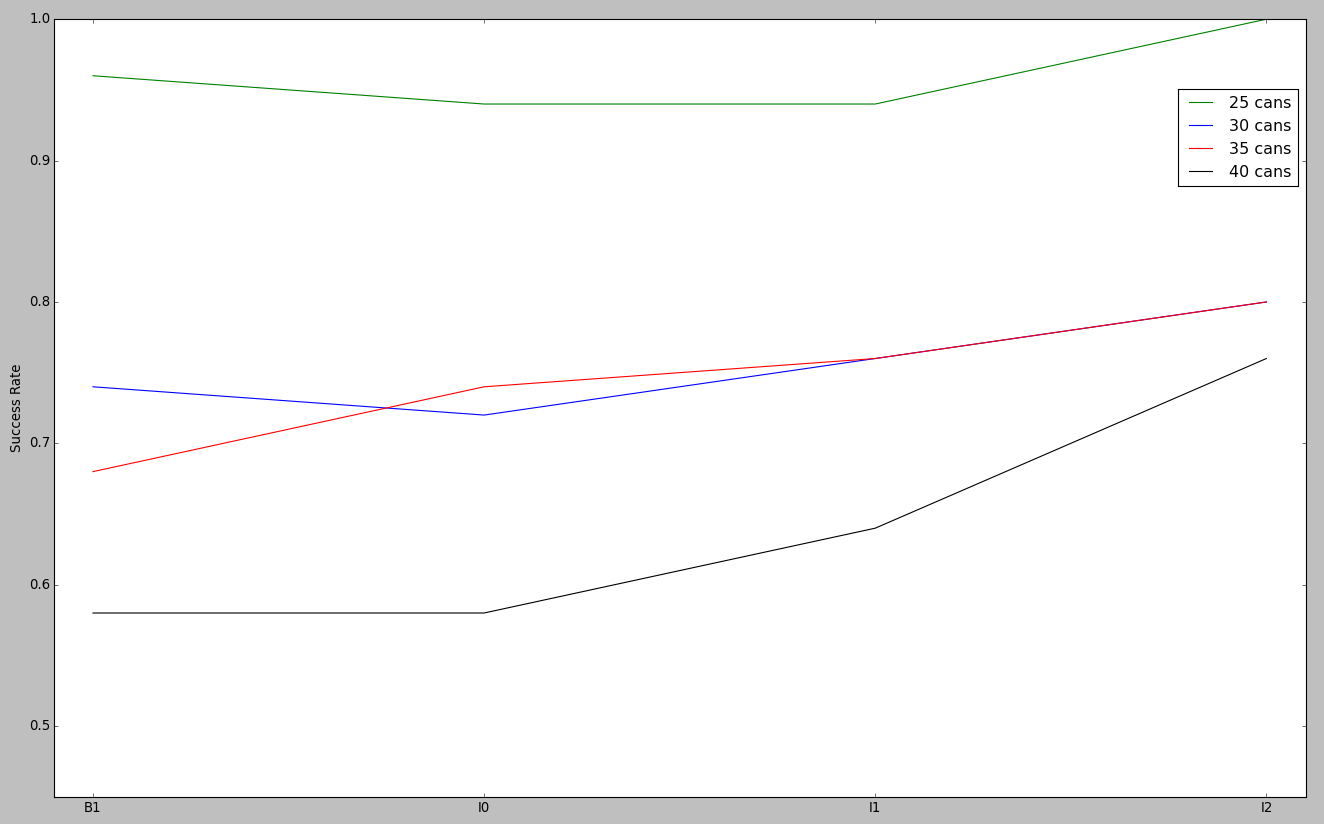
\includegraphics[scale=0.43]{images/results_line.png}
  \caption{\small{Line graph illustrating success rates on the test set for baseline 1
and our system after each round of DAgger, using the abbreviations described in the
table caption. Our method performs much better than the baseline after 2 iterations of DAgger.
We also note the upward trend in success rate across the iterations.}}
  \label{fig:results_line}
\end{figure}

\begin{figure}[h]
  \centering
    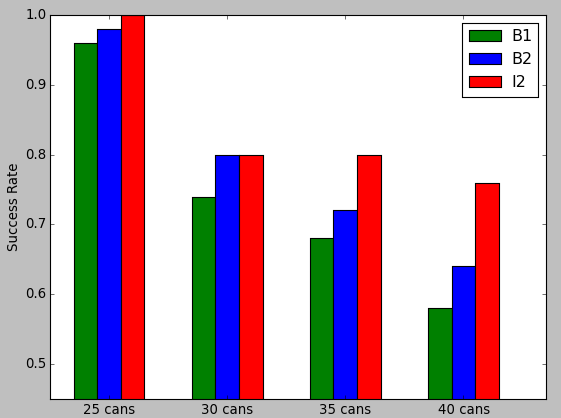
\includegraphics[scale=0.43]{images/results_bar_succ.png}
  \caption{\small{Bar graph illustrating success rates on the test set for the
two baselines and our system after 2 iterations of DAgger. Our method achieved much higher
success rates than both baselines, in general.}}
  \label{fig:results_bar_succ}
\end{figure}

\begin{figure}[h]
  \centering
    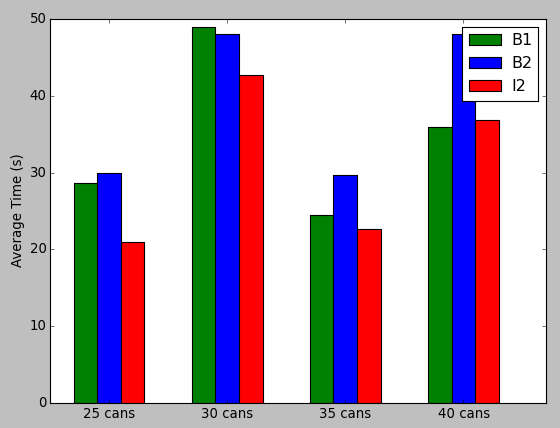
\includegraphics[scale=0.43]{images/results_bar_time.png}
  \caption{\small{Bar graph illustrating average total times on the test set for the
two baselines and our system after 2 iterations of DAgger. Our method produced noticeably faster
performance than both baselines, in general.}}
  \label{fig:results_bar_time}
\end{figure}

We run four sets of experiments, using 25, 30, 35, and 40 cans on the table.
The goal across all experiments is for the robot to pick up a particular object with its
left gripper. We disabled the right gripper, so any obstructions to the target object must be picked up and
placed elsewhere on the table. This domain has 4 types of continuous references: base poses, object grasp
poses, object putdown poses, and object putdown locations onto the table.

We now describe the feature vector $f(n)$ associated with a high-level plan. Because the plan is composed
of a sequence of object grasp and putdown actions, we first consider features of a single grasp action, targeted
at an object $o$ in the environment. Consider a cone ranging from angles $-\frac{\pi}{3}$ to $\frac{\pi}{3}$
toward the closest table edge from $o$, as shown in \figref{fig:cone}. The first feature, exists\_obstr, is a binary variable indicating
whether any other objects lie in this cone. The second, exists\_path, is a binary variable indicating whether there is a linear
grasp path wide enough for the robot's gripper to fit through within the cone. The third, sweep\_count, sweeps
a cylinder $c$ approximating the robot's gripper across 10 discretized angles from $-\frac{\pi}{3}$ to
$\frac{\pi}{3}$ and is the minimum number of objects in collision with $c$ across these angles.
We construct these features for the first five grasp actions in the plan (padding with -1 if there are not enough).
We then add on the following aggregate features associated with the entire plan: 1) the minimum exists\_obstr across grasp actions,
2) the sum of sweep\_count across grasp actions, 3) a counter for how many times $n$ was picked for refinement, and
4) a counter for how many times $n$ was picked for generating an error.

We report results on fixed test sets of 50 randomly generated environments per number of objects. At each
iteration of training, we collect approximately 100 optimal actions from the human demonstrator (using
DAgger, this means collect 100 demonstrations, construct $w$, collect 100 more while rolling out $w$, construct new $w$, repeat).
We found that after 2 rounds of DAgger, performance plateaued, so we stopped there.

Our experiments are conducted in Python 2.7 using the OpenRave simulator~\cite{Diankov_2008_6117} with a PR2 robot.
The motion planner we use is trajopt~\cite{schulman2013finding}, and the task planner is Fast-Forward~\cite{FF}.
The experiments were carried out in series on an Intel Core i7-4770K machine with 16GB RAM. For the max-margin optimization,
we used a constant margin of $d = 1$, and we set $C = 10^{9}$, indicating that we want to penalize violating
constraints significantly and are willing to have $||w||$ be large. In our experiments, though, $||w||$ did not actually become
large. We used Gurobi as our optimizer for solving the quadratic program.

Table \ref{table:results} summarizes our quantitative results. \figref{fig:cover} illustrates a scenario where
our learning methods prove important. \figref{fig:results_line}, \figref{fig:results_bar_succ}, and \figref{fig:results_bar_time} show our quantitative
results in graphs. The results demonstrate significant improvements in performance to the baseline systems for success rate and
average overall time. The number of calls to the motion planner remained roughly the same,
suggesting that the performance benefits instead derive from less time wasted on inverse kinematics checks when
attempting to refine plans with no valid refinement.
